\documentclass{beamer}
\usetheme{Singapore}
\usepackage{changepage}

%\usepackage{pstricks,pst-node,pst-tree}
\usepackage{amssymb,latexsym}
\usepackage{tikz}
\usepackage{graphicx}
\usepackage{fancyvrb}
\usepackage{hyperref}
\usepackage{fancybox}

\newcommand{\bi}{\begin{itemize}}
\newcommand{\li}{\item}
\newcommand{\ei}{\end{itemize}}
\newcommand{\Show}[1]{
\begin{center}
\shadowbox{\begin{minipage}{0.8\textwidth}
          \bf #1
          \end{minipage}}
\end{center}
}
\newcommand{\arrow}{\ensuremath{\rightarrow}}

\newcommand{\uparr}{\ensuremath{\uparrow}}


\newcommand{\fig}[2]{\centerline{\includegraphics[width=#1\textwidth]{#2}}}

\newcommand{\figg}[2]{\includegraphics[width=#1\textwidth]{#2}}

\newcommand{\bfr}[1]{\begin{frame}[fragile]\frametitle{{ #1 }}}
\newcommand{\efr}{\end{frame}}

\newcommand{\cola}[1]{\begin{columns}\begin{column}{#1\textwidth}}
\newcommand{\colb}[1]{\end{column}\begin{column}{#1\textwidth}}
\newcommand{\colc}{\end{column}\end{columns}}


\author{Fundamentals of Data Visualization}
\title{Chapter 27\\Image file formats}

\begin{document}

\begin{frame}
\maketitle
\end{frame}

\bfr{Bitmap vs. Vector}
\fig{1.1}{bitmap-zoom-1}
\bi
\li Vector graphics always sharp
\li Vector graphics can be enormous for large data sets
\li Vector graphics can be very small for small data sets
\ei
\end{frame}

\bfr{Common formats}
\fig{1.1}{formattable}
Recommendations:
\bi
\li Vector: pdf
\li Bitmap: png
\li Very large bitmap: jpeg
\ei
\end{frame}


\bfr{Lossless and lossy compression of bitmaps}

\centerline{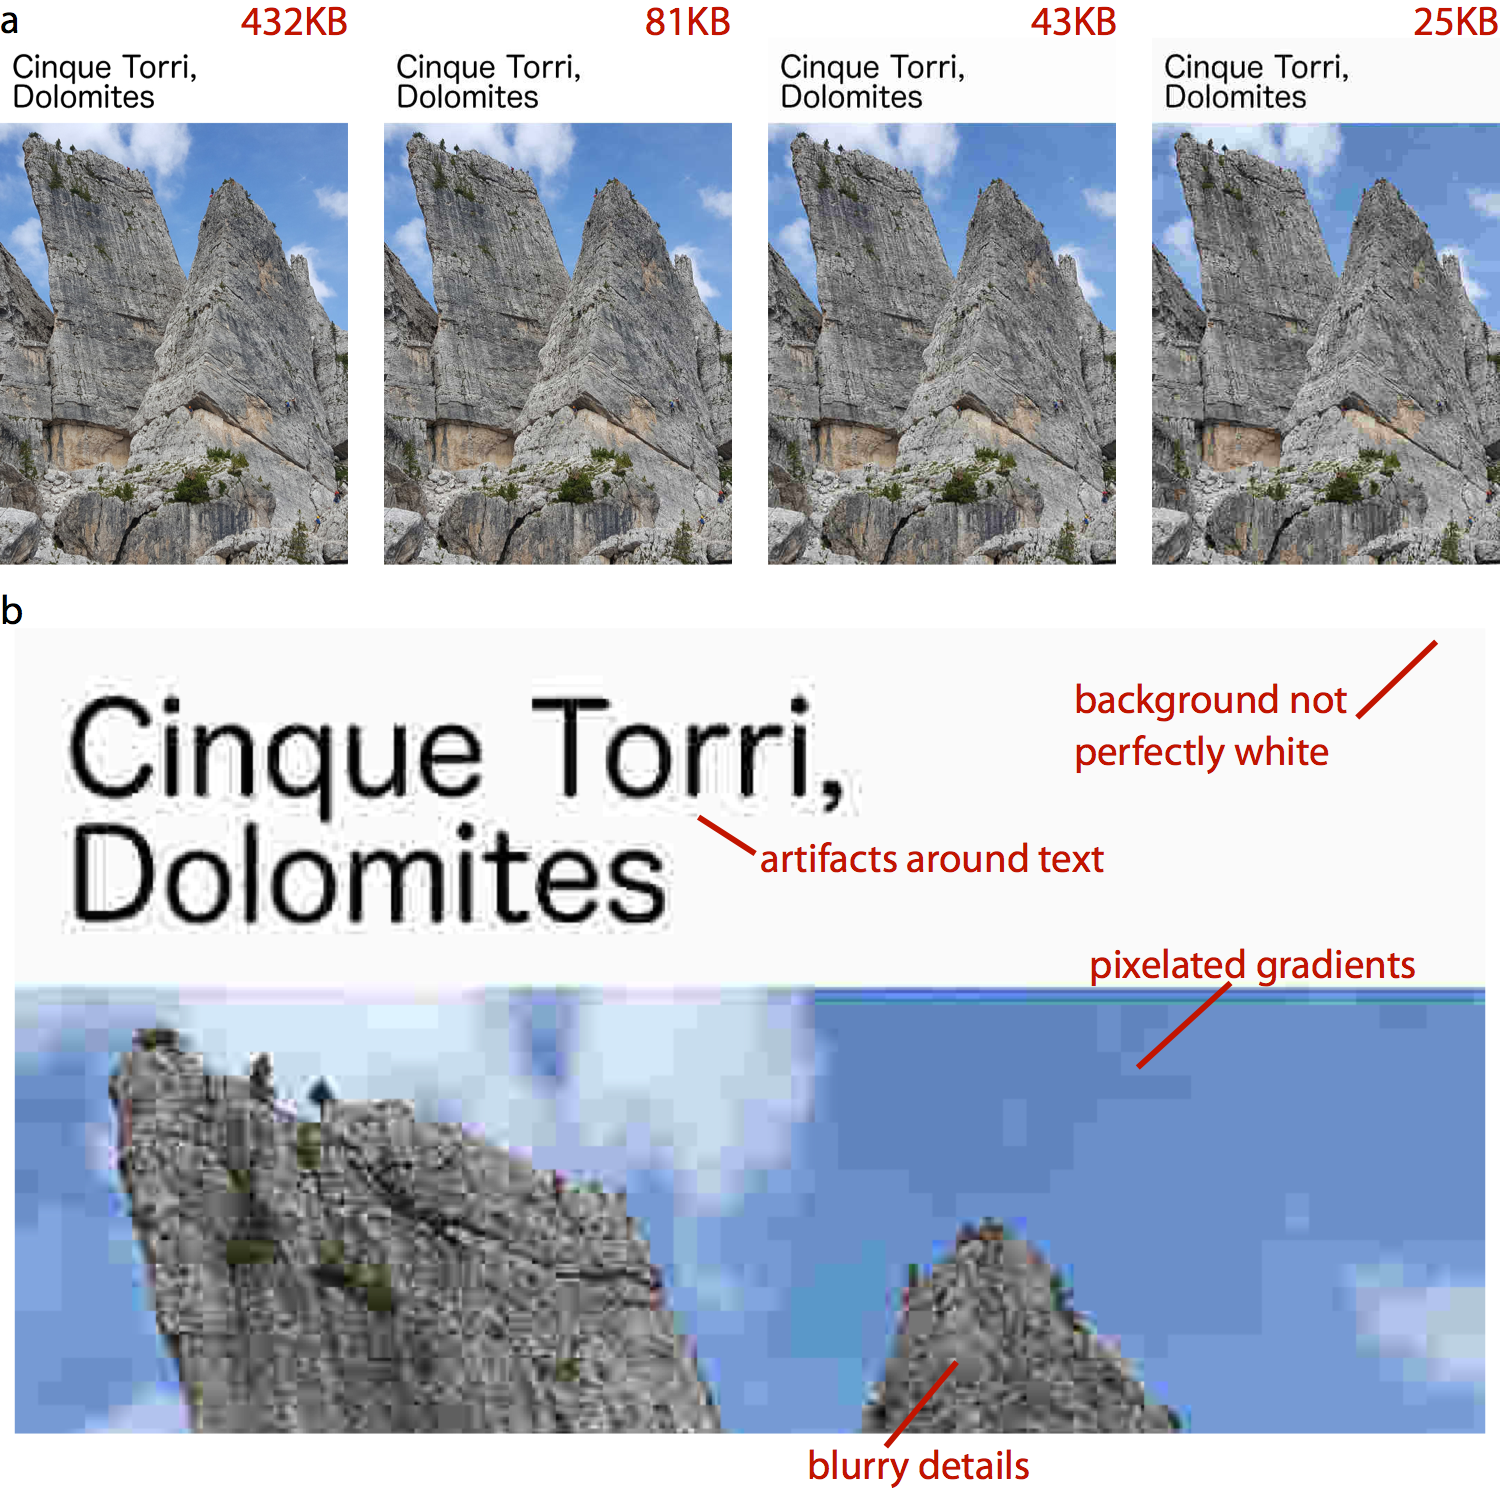
\includegraphics[trim={0 4.5in 0 0},clip,width=1.1\textwidth]{jpeg_example_combined.png}}
\end{frame}

\bfr{Lossless and lossy compression of bitmaps}

\centerline{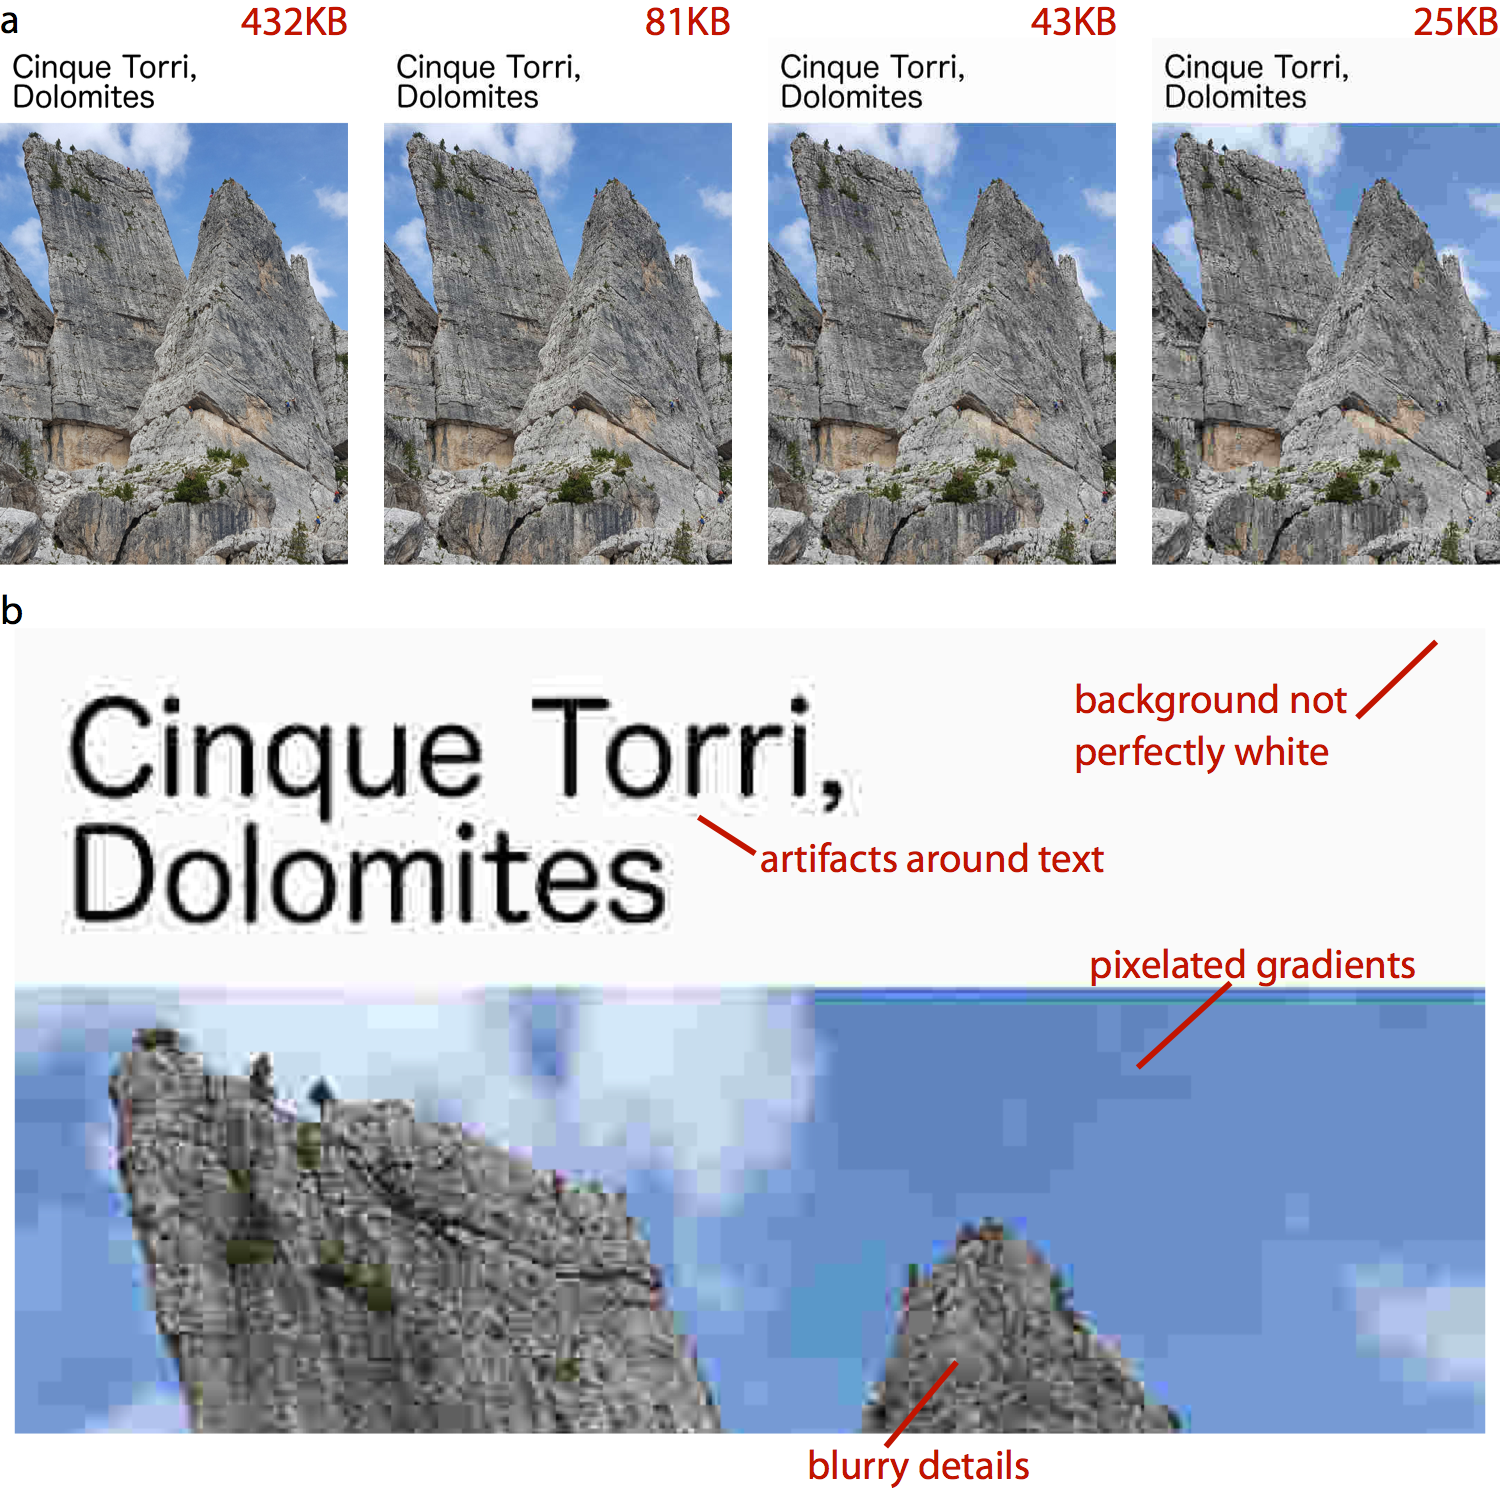
\includegraphics[trim={0 0 0 3in},clip,width=1.1\textwidth]{jpeg_example_combined.png}}
\end{frame}

\bfr{Converting between image formats}
\bi
\li Can lose information
\bi
\li vector to bitmap
\li lossless to lossy
\ei
\li Always store the original image in the format that maintains maximum resolution, accuracy, and flexibility
\li PDF for data visualizations, or source code
\li Store bitmaps in as high a resolution as possible, losslessly
\li Convert these as necessary
\ei
\end{frame}


\end{document}
